% Options for packages loaded elsewhere
\PassOptionsToPackage{unicode}{hyperref}
\PassOptionsToPackage{hyphens}{url}
%
\documentclass[
  ignorenonframetext,
]{beamer}
\usepackage{pgfpages}
\setbeamertemplate{caption}[numbered]
\setbeamertemplate{caption label separator}{: }
\setbeamercolor{caption name}{fg=normal text.fg}
\beamertemplatenavigationsymbolsempty
% Prevent slide breaks in the middle of a paragraph
\widowpenalties 1 10000
\raggedbottom
\setbeamertemplate{part page}{
  \centering
  \begin{beamercolorbox}[sep=16pt,center]{part title}
    \usebeamerfont{part title}\insertpart\par
  \end{beamercolorbox}
}
\setbeamertemplate{section page}{
  \centering
  \begin{beamercolorbox}[sep=12pt,center]{part title}
    \usebeamerfont{section title}\insertsection\par
  \end{beamercolorbox}
}
\setbeamertemplate{subsection page}{
  \centering
  \begin{beamercolorbox}[sep=8pt,center]{part title}
    \usebeamerfont{subsection title}\insertsubsection\par
  \end{beamercolorbox}
}
\AtBeginPart{
  \frame{\partpage}
}
\AtBeginSection{
  \ifbibliography
  \else
    \frame{\sectionpage}
  \fi
}
\AtBeginSubsection{
  \frame{\subsectionpage}
}
\usepackage{lmodern}
\usepackage{amssymb,amsmath}
\usepackage{ifxetex,ifluatex}
\ifnum 0\ifxetex 1\fi\ifluatex 1\fi=0 % if pdftex
  \usepackage[T1]{fontenc}
  \usepackage[utf8]{inputenc}
  \usepackage{textcomp} % provide euro and other symbols
\else % if luatex or xetex
  \usepackage{unicode-math}
  \defaultfontfeatures{Scale=MatchLowercase}
  \defaultfontfeatures[\rmfamily]{Ligatures=TeX,Scale=1}
\fi
% Use upquote if available, for straight quotes in verbatim environments
\IfFileExists{upquote.sty}{\usepackage{upquote}}{}
\IfFileExists{microtype.sty}{% use microtype if available
  \usepackage[]{microtype}
  \UseMicrotypeSet[protrusion]{basicmath} % disable protrusion for tt fonts
}{}
\makeatletter
\@ifundefined{KOMAClassName}{% if non-KOMA class
  \IfFileExists{parskip.sty}{%
    \usepackage{parskip}
  }{% else
    \setlength{\parindent}{0pt}
    \setlength{\parskip}{6pt plus 2pt minus 1pt}}
}{% if KOMA class
  \KOMAoptions{parskip=half}}
\makeatother
\usepackage{xcolor}
\IfFileExists{xurl.sty}{\usepackage{xurl}}{} % add URL line breaks if available
\IfFileExists{bookmark.sty}{\usepackage{bookmark}}{\usepackage{hyperref}}
\hypersetup{
  pdftitle={Governing through Patronage},
  pdfauthor={Galileu Kim},
  hidelinks,
  pdfcreator={LaTeX via pandoc}}
\urlstyle{same} % disable monospaced font for URLs
\newif\ifbibliography
\setlength{\emergencystretch}{3em} % prevent overfull lines
\providecommand{\tightlist}{%
  \setlength{\itemsep}{0pt}\setlength{\parskip}{0pt}}
\setcounter{secnumdepth}{-\maxdimen} % remove section numbering
\usetheme{Malmoe}

% packages
% \usepackage{attachfile}
\useoutertheme{infolines} % Alternatively: miniframes, infolines, split
\useinnertheme{circles}

% colors
\definecolor{princeton}{rgb}{1.0, 0.6, 0.2} % princeton (primary)
\definecolor{arsenic}{rgb}{0.23, 0.27, 0.29}

\setbeamercolor{title}{fg=black}
\setbeamercolor{frametitle}{fg=white,bg=arsenic}
\setbeamercolor{section in head/foot}{fg=arsenic,bg=princeton}
\setbeamerfont{frametitle}{size=\Large}
%\setbeamercolor{palette primary}{bg=princeton,fg=black}
%\setbeamercolor{palette secondary}{bg=princeton,fg=black}
%\setbeamercolor{palette tertiary}{bg=princeton,fg=black}
%\setbeamercolor{palette quaternary}{bg=princeton,fg=black}
\setbeamercolor{structure}{fg=princeton} % itemize, enumerate, etc
\setbeamercolor{section in toc}{fg=arsenic} % TOC sections
\setbeamerfont{subtitle}{size=\small}

% override palette coloring with secondary
\setbeamercolor{subsection in head/foot}{bg=arsenic,fg=white}

% defining font
\usepackage[T1]{fontenc}

% Cabin
\usepackage[sfdefault,condensed]{cabin}

% Helvetica
%\usepackage[scaled]{helvet}
%\renewcommand\familydefault{\sfdefault}

% Inria Sans
%\usepackage[lining]{InriaSans}
%\renewcommand*\oldstylenums[1]{{\fontfamily{InriaSans-OsF}\selectfont #1}}
%% The font package uses mweights.sty which has som issues with the
%% \normalfont command. The following two lines fixes this issue.
%\let\oldnormalfont\normalfont
%\def\normalfont{\oldnormalfont\mdseries}

% FiraSans
%\usepackage[sfdefault]{FiraSans}
%\renewcommand*\oldstylenums[1]{{\firaoldstyle #1}}
%\usepackage{ragged2e}

% set margins
\setbeamersize{text margin left=10mm,text margin right=10mm}

% source command
\newcommand{\source}{\footnotesize\textcolor{black!25}}

% suppress section slides
\AtBeginSubsection{}
\AtBeginSection{}

\title{Governing through Patronage}
\subtitle{the Bargain for Education in Decentralized Brazil}
\author{Galileu Kim}
\date{2019-11-13}

\begin{document}
\frame{\titlepage}

\hypertarget{motivation}{%
\section{Motivation}\label{motivation}}

\begin{frame}{A tale of two schools}
\protect\hypertarget{a-tale-of-two-schools}{}

\begin{center}\includegraphics[width=160px]{/home/gali/princeton/dissertation/thesis/presentation/presentation_plas/figs/photo_cover_plas_2019} \end{center}

\end{frame}

\begin{frame}{Expansion in public education}
\protect\hypertarget{expansion-in-public-education}{}

\begin{itemize}
\tightlist
\item
  Across the world, children rely on public education.
\item
  Rapid expansion in coverage over the last decades.
\item
  Improvements in \emph{quality} remain a challenge.
\end{itemize}

\end{frame}

\begin{frame}{Net primary enrollment rates}
\protect\hypertarget{net-primary-enrollment-rates}{}

\begin{center}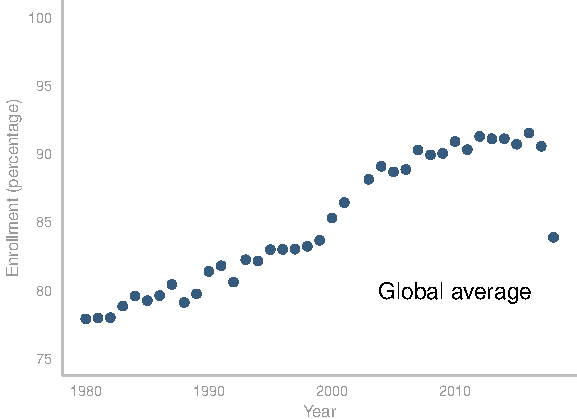
\includegraphics{presentation_plas_11-14-19_files/figure-beamer/unnamed-chunk-2-1} \end{center}

\end{frame}

\begin{frame}{Net primary enrollment rates}
\protect\hypertarget{net-primary-enrollment-rates-1}{}

\begin{center}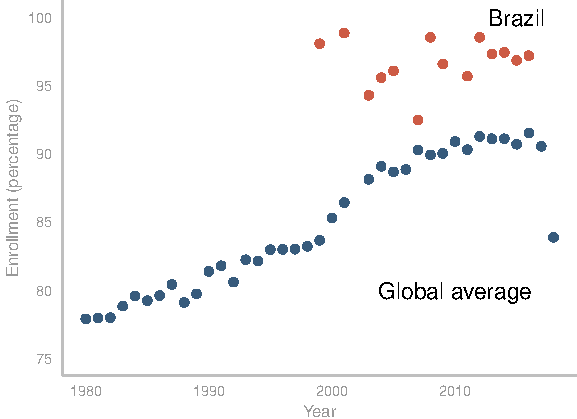
\includegraphics{presentation_plas_11-14-19_files/figure-beamer/unnamed-chunk-3-1} \end{center}

\end{frame}

\begin{frame}{Quality of education}
\protect\hypertarget{quality-of-education}{}

\begin{center}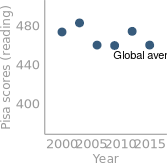
\includegraphics{presentation_plas_11-14-19_files/figure-beamer/unnamed-chunk-4-1} \end{center}

\end{frame}

\begin{frame}{Quality of education}
\protect\hypertarget{quality-of-education-1}{}

\begin{center}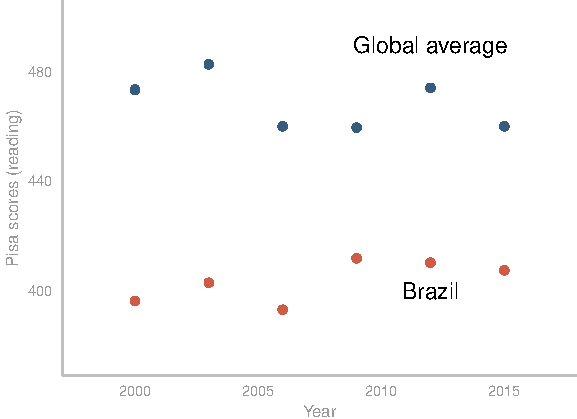
\includegraphics{presentation_plas_11-14-19_files/figure-beamer/unnamed-chunk-5-1} \end{center}

\end{frame}

\begin{frame}{A domestic story}
\protect\hypertarget{a-domestic-story}{}

\begin{figure}

{\centering 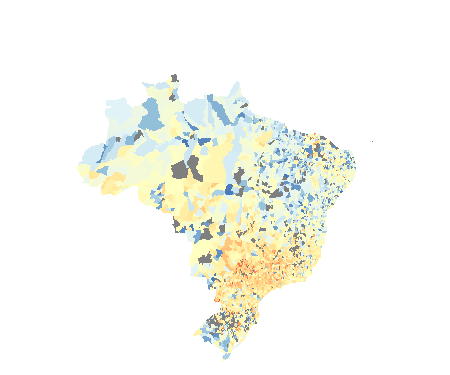
\includegraphics{figs/saeb_map} 

}

\caption{Source: National System for Educational Assessment (SAEB)}\label{fig:unnamed-chunk-6}
\end{figure}

\end{frame}

\begin{frame}{Research question}
\protect\hypertarget{research-question}{}

\begin{itemize}
\tightlist
\item
  Why does inequality in the quality of public education persist? Why do
  some communities have access to better quality education than others?
\item
  How do local actors decide to manage public education? What are the
  political costs and benefits of improving public education?
\end{itemize}

\end{frame}

\begin{frame}{Findings}
\protect\hypertarget{findings}{}

\begin{itemize}
\tightlist
\item
  Bureaucratic staff turnover has negative consequences for student
  learning.
\item
  Staff positions granted to members of legislative coalition.
\item
  Political fragmentation leads to greater patronage.
\item
  Electoral accountability does not bite: elite game.
\end{itemize}

\end{frame}

\begin{frame}{Outline}
\protect\hypertarget{outline}{}

\tableofcontents

\end{frame}

\hypertarget{the-debate}{%
\section{The debate}\label{the-debate}}

\begin{frame}{Public services provision}
\protect\hypertarget{public-services-provision}{}

\end{frame}

\hypertarget{the-case}{%
\section{The case}\label{the-case}}

\begin{frame}{The case: Brazil}
\protect\hypertarget{the-case-brazil}{}

\begin{itemize}
\tightlist
\item
  Over 23 million students enrolled in public schools.
\item
  \textasciitilde12\% of GDP spent in education.
\item
  1.2 million public teachers per year.
\item
  5.5 thousand municipalities.
\item
  Education is local: municipal governments administer primary
  education.
\end{itemize}

\end{frame}

\begin{frame}{Data}
\protect\hypertarget{data}{}

\begin{itemize}
\tightlist
\item
  Student learning.

  \begin{itemize}
  \tightlist
  \item
    National System of Educational Assessment (SAEB)
  \item
    Ceará System of Learning Assessment (SPAECE)
  \end{itemize}
\item
  Educational staff.

  \begin{itemize}
  \tightlist
  \item
    National School Census
  \item
    Annual Report on Social Information (RAIS)
  \end{itemize}
\item
  Additional covariates.

  \begin{itemize}
  \tightlist
  \item
    National Institute of Geography and Statistics (IBGE)
  \item
    FINBRA
  \item
    TSE
  \end{itemize}
\end{itemize}

\end{frame}

\begin{frame}{Alternative explanations}
\protect\hypertarget{alternative-explanations}{}

\begin{center}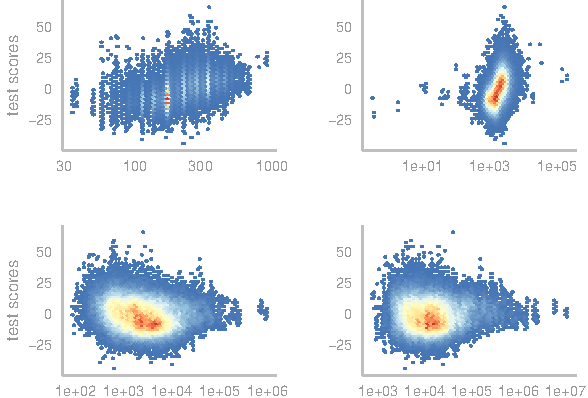
\includegraphics{presentation_plas_11-14-19_files/figure-beamer/unnamed-chunk-7-1} \end{center}

\end{frame}

\hypertarget{the-argument}{%
\section{The argument}\label{the-argument}}

\begin{frame}{Movement in two steps}
\protect\hypertarget{movement-in-two-steps}{}

\begin{itemize}
\tightlist
\item
  Quality of student learning decreases with educational staff turnover.
\item
  Teacher and school principals are reshuffled as a result of political
  turnover.
\item
  Jobs are allocated to coalition members, to maintain legislative
  support.
\item
  An elite game: electoral accountability does not bite.
\end{itemize}

\end{frame}

\begin{frame}{Educational staff turnover}
\protect\hypertarget{educational-staff-turnover}{}

\begin{center}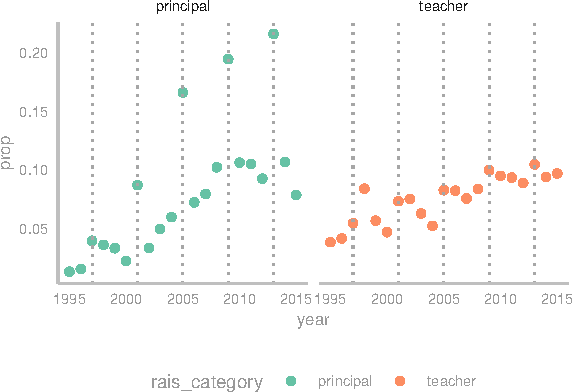
\includegraphics{presentation_plas_11-14-19_files/figure-beamer/unnamed-chunk-8-1} \end{center}

\end{frame}

\begin{frame}{Table of contents}
\protect\hypertarget{table-of-contents}{}

\begin{center}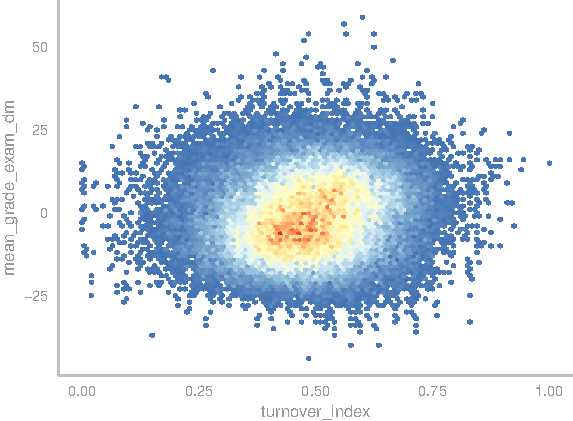
\includegraphics{presentation_plas_11-14-19_files/figure-beamer/unnamed-chunk-9-1} \end{center}

\end{frame}

\hypertarget{results}{%
\section{Results}\label{results}}

\begin{frame}{First stage}
\protect\hypertarget{first-stage}{}

\end{frame}

\begin{frame}{Second stage}
\protect\hypertarget{second-stage}{}

\end{frame}

\hypertarget{conclusion}{%
\section{Conclusion}\label{conclusion}}

\end{document}
